% This LaTeX document needs to be compiled with XeLaTeX.
\documentclass[10pt]{article}
\usepackage[utf8]{inputenc}
\usepackage{amsmath}
\usepackage{amsfonts}
\usepackage{amssymb}
\usepackage[version=4]{mhchem}
\usepackage{stmaryrd}
\usepackage{graphicx}
\usepackage[export]{adjustbox}
\graphicspath{ {./images/} }
\usepackage[fallback]{xeCJK}
\usepackage{polyglossia}
\usepackage{fontspec}
\setCJKmainfont{Noto Serif CJK JP}

\setmainlanguage{polish}
\setmainfont{CMU Serif}

\title{LIGA MATEMATYCZNA im. Zdzisława Matuskiego \\
 PÓŁFINAモ }

\author{}
\date{}


\begin{document}
\maketitle
\section*{7 lutego 2013}
GIMNAZJUM

\section*{ZADANIE 1.}
Kwadraty \(A C E G, B C D I\), \(J F G H\) mają pola równe odpowiednio \(3600 \mathrm{~cm}^{2}, 900 \mathrm{~cm}^{2}\) oraz \(400 \mathrm{~cm}^{2}\). Oblicz pole trójkąta AIJ.\\
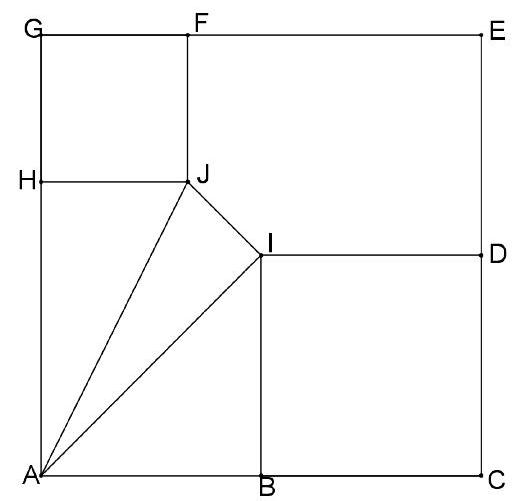
\includegraphics[max width=\textwidth, center]{2024_11_21_63b5750d3d350075f4b4g-1}

\section*{ZADANIE 2.}
W ułamku

\[
\frac{1 \cdot 2 \cdot 3 \cdot \ldots \cdot 23}{1-2+3-4+5-6+\ldots+203}
\]

licznik jest iloczynem kolejnych liczb naturalnych od 1 do 23, natomiast w mianowniku kolejne liczby naturalne od 1 do 203 są naprzemian odejmowane i dodawane. Czy wartość tego ułamka jest liczbą całkowitą?

\section*{ZADANIE 3.}
Na boku \(C D\) prostokąta \(A B C D\) wybrano punkt \(E\) w taki sposób, że trapez \(A B C E\) ma pole równe \(57,5 \mathrm{~cm}^{2}\), a pole trapezu \(A B E D\) jest równe \(70 \mathrm{~cm}^{2}\). Oblicz pole prostokąta \(A B C D\).

\section*{ZADANIE 4.}
Porównaj liczby \(\frac{a}{a-1}\) oraz \(\frac{b}{b-1}\), gdy \(a\) i \(b\) spełniają warunek \(1<a<b\).

\section*{ZADANIE 5.}
Wykaż, że liczba \(n^{3}+23 n\) jest podzielna przez 6 dla każdej liczby naturalnej \(n\).


\end{document}